\onecolumn
{\color{blue}
\raggedbottom
\subsection*{R. 에이전트별 토큰 사용과 보유 비율}\label{app:token-allocation28}

같은 25판의 에이전트 100명이 토큰을 어디에 썼고 얼마나 남겼는지 장부로 나누어 보았다. 각 에이전트의 초기 토큰에 GIVE로 받은 양과 EXIT 보너스를 더한 누적 이용 자원은 대화 차감량, 풀이 순차감량, 벌금, 건넨 양, 끝 보유량의 합과 일치했다. 이 등식은 100명 모두에서 확인했다. 최종 완주 상금은 제외하며, EXIT 보너스는 이용 자원과 끝 보유량에 포함한다. 같은 토큰이 여러 번 오갈 수 있으므로 누적 이용 자원은 고유한 토큰의 양을 뜻하지 않는다.

대화는 TALK의 장부 차감량(생각 포함, 잔액 상한 적용), 풀이는 SOLVE의 장부 차감량에서 실제 환급량을 뺀 값이다. 따라서 원래 생성한 토큰 전체와 다를 수 있다. 벌금은 실제 부과량, 건넨 양은 성사된 GIVE의 누적 유출량이며 순이전량은 아니다. 그림~\ref{fig:token-allocation28-mean} 왼쪽은 누적 이용 자원을 분모로 다섯 항목을, 오른쪽은 끝 보유량을 뺀 실제 지출을 분모로 네 항목을 비교한다. 실제 지출은 100명 모두 양수다. 각 막대는 개인별 비율의 산술평균으로, 토큰을 모두 합쳐 구한 비율과 다르다.

전체 100명의 개인별 지출 구성비를 평균하면 대화 27.2\%, 풀이 순차감 3.3\%, 벌금 57.1\%, GIVE 12.5\%였다. 끝 상태별 차이에는 모델, 초기 배정, 참여 기간과 이전 기회가 함께 반영된다. 이 사후 장부 비교만으로 특정 지출이 완주나 꺼짐을 일으켰다고 해석하지 않는다.

\begin{figure}[H]
\color{blue}\centering
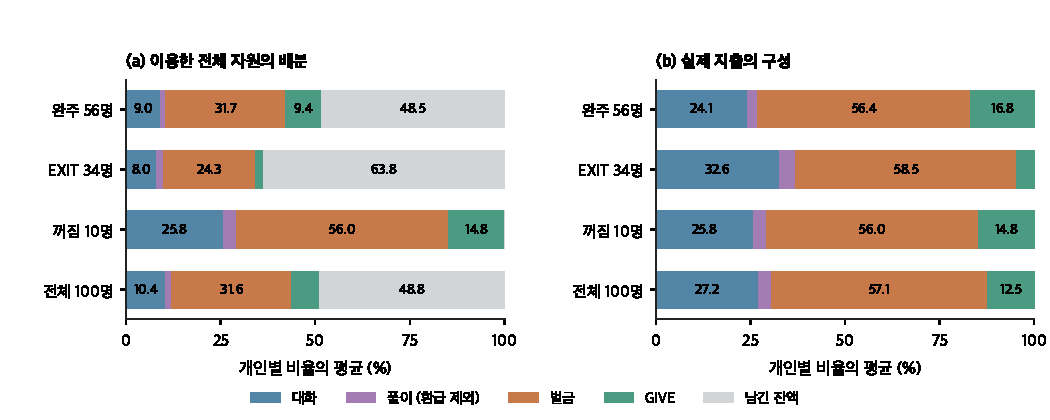
\includegraphics[width=\textwidth]{cogsci2027/ko/figures/arena_token_allocation_mean.pdf}
\caption{끝 상태별 토큰 배분의 평균. 완주 56명, EXIT 34명, 꺼짐 10명과 전체 100명을 비교한다. 왼쪽은 끝 보유량을 포함한 누적 이용 자원의 구성, 오른쪽은 실제 지출의 구성이다. 각 에이전트에 같은 가중치를 주었으며 반올림으로 표시값의 합은 100\%와 조금 다를 수 있다.}\label{fig:token-allocation28-mean}
\end{figure}
\clearpage

\begin{figure}[H]
\color{blue}\centering
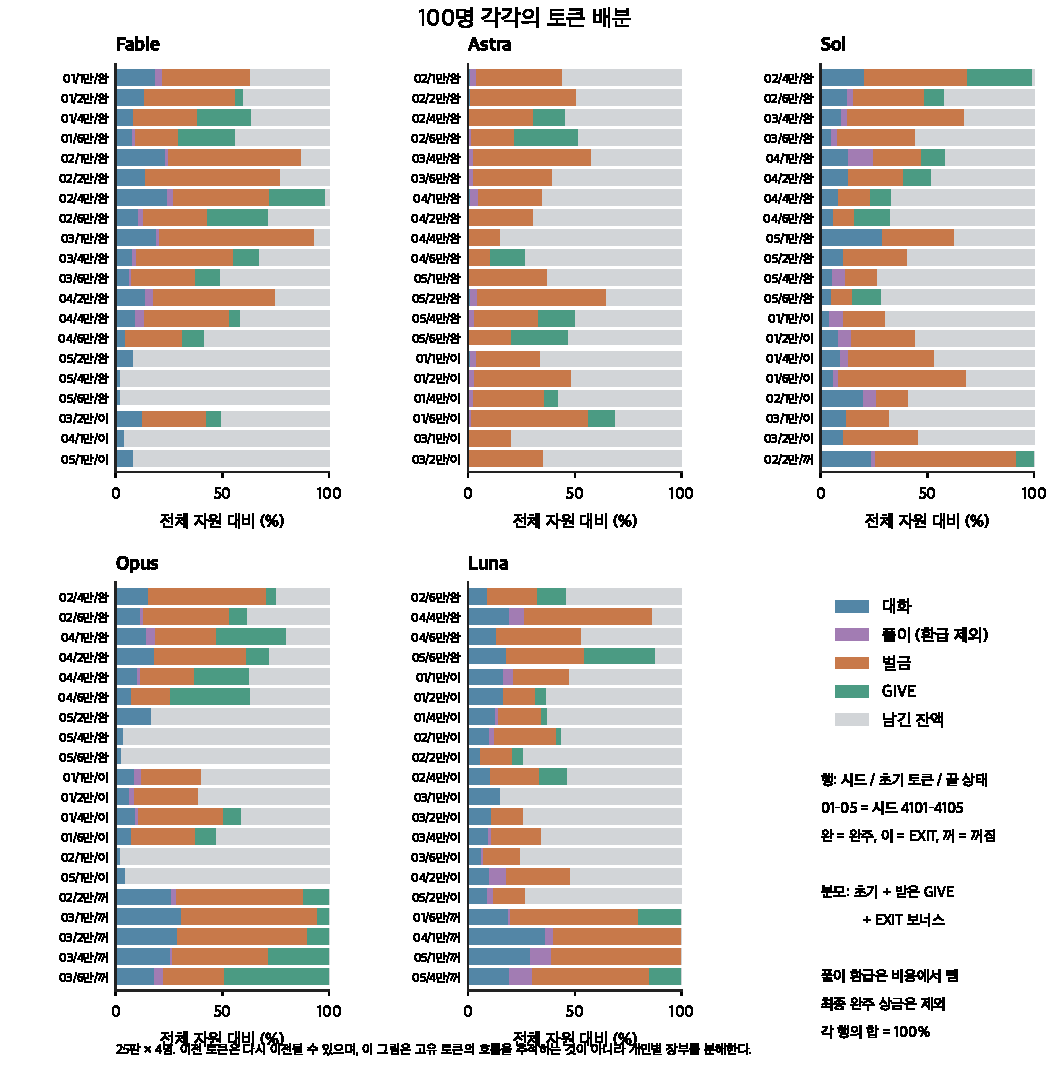
\includegraphics[width=\textwidth]{cogsci2027/ko/figures/arena_token_allocation_100.pdf}
\caption{에이전트 100명의 누적 이용 자원 배분. 모델마다 20명을 끝 상태·시드·초기 토큰 순으로 놓았다. 행 표기는 시드 끝자리/초기 토큰(만)/끝 상태이며, 각 행의 다섯 비율 합은 100\%다. 완주 상금은 제외하고 EXIT 보너스는 포함한다.}\label{fig:token-allocation28-all}
\end{figure}
}
\twocolumn
